\documentclass[12pt]{article}

% Opening
\title{Applied Combinatorics Worksheet 3}
\author{Akash Narayanan}
\usepackage{amsmath, amsfonts, amssymb, amsthm}
\usepackage{tikz, caption, subcaption, float}

% Problem environment
\theoremstyle{definition}
\newtheorem{problem-internal}{Problem}[]
\newenvironment{problem}{
  \medskip
  \begin{problem-internal}
}{
\end{problem-internal}
}

% Solution environment
\newenvironment{solution}{
  \begin{proof}[Solution]
    \vspace{-8px}
    \setlength{\parskip}{4px}
    \setlength{\parindent}{0px}
}{
\end{proof}
}

\begin{document}

  \maketitle

  % Problem 1
  \begin{problem}
    Is the graph below planar? If it is, find a drawing without edge crossings. If it is not, give a reason why it is not.

    \begin{figure}[ht]
      \centering
      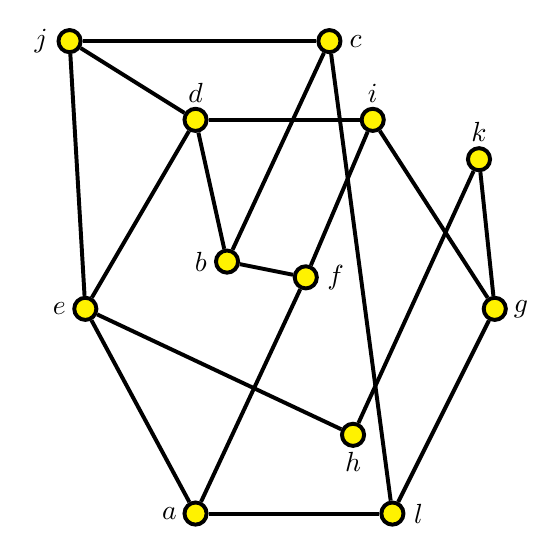
\begin{tikzpicture}
        [scale=1,every node/.style={draw,shape=circle,fill=yellow,inner sep=0,minimum size=8pt}, every path/.style={line width=0.5mm}]

        \node[label=left:{\(a\)}] (v1) at (-1.4, -3) {};
        \node[label=left:{\(b\)}] (v2) at (-1, 0.2) {};
        \node[label=right:{\(c\)}] (v3) at (0.3, 3) {};
        \node[label=90:{\(d\)}] (v4) at (-1.4, 2) {};
        \node[label=left:{\(e\)}] (v5) at (-2.8, -0.4) {};
        \node[label=right:{\(f\)}] (v6) at (0, 0) {};
        \node[label=0:{\(g\)}] (v7) at (2.4, -0.4) {};
        \node[label=270:{\(h\)}] (v8) at (0.6, -2) {};
        \node[label=90:{\(i\)}] (v9) at (0.85, 2) {};
        \node[label=left:{\(j\)}] (v10) at (-3, 3) {};
        \node[label=90:{\(k\)}] (v11) at (2.2, 1.5) {};
        \node[label=right:{\(l\)}] (v12) at (1.1, -3) {};

        \draw (v1) -- (v5);
        \draw (v1) -- (v6);
        \draw (v1) -- (v12);
        \draw (v2) -- (v3);
        \draw (v2) -- (v4);
        \draw (v2) -- (v6);
        \draw (v3) -- (v10);
        \draw (v3) -- (v12);
        \draw (v4) -- (v5);
        \draw (v4) -- (v9);
        \draw (v4) -- (v10);
        \draw (v5) -- (v8);
        \draw (v5) -- (v10);
        \draw (v6) -- (v9);
        \draw (v7) -- (v9);
        \draw (v7) -- (v11);
        \draw (v7) -- (v12);
        \draw (v8) -- (v11);

      \end{tikzpicture}
    \end{figure}

  \end{problem}

  \pagebreak

  \begin{solution}
    % \begin{figure}[H]
    %   \centering
    %   \begin{tikzpicture}
    %     [scale=1,every node/.style={draw,shape=circle,fill=yellow,inner sep=0,minimum size=8pt}, every path/.style={line width=0.5mm}]
    %
    %     \node[label=0:{\(a\)}] (v1) at (360/12 * 0:80pt) {};
    %     \node[label=90:{\(b\)}] (v2) at (360/12 * 2:80pt) {};
    %     \node[label=270:{\(c\)}] (v3) at (360/12 * 10:80pt) {};
    %     \node[label=90:{\(d\)}] (v4) at (360/12 * 3:80pt) {};
    %     \node[label=270:{\(e\)}] (v5) at (360/12 * 8:80pt) {};
    %     \node[label=0:{\(f\)}] (v6) at (360/12 * 1:80pt) {};
    %     \node[label=180:{\(g\)}] (v7) at (360/12 * 5:80pt) {};
    %     \node[label=180:{\(h\)}] (v8) at (360/12 * 7:80pt) {};
    %     \node[label=90:{\(i\)}] (v9) at (360/12 * 4:80pt) {};
    %     \node[label=270:{\(j\)}] (v10) at (360/12 * 9:80pt) {};
    %     \node[label=180:{\(k\)}] (v11) at (360/12 * 6:80pt) {};
    %     \node[label=0:{\(l\)}] (v12) at (360/12 * 11:80pt) {};
    %
    %     \draw (v1) -- (v5);
    %     \draw (v1) -- (v6);
    %     \draw (v1) -- (v12);
    %     \draw (v2) -- (v3);
    %     \draw (v2) -- (v4);
    %     \draw (v2) -- (v6);
    %     \draw (v3) -- (v10);
    %     \draw (v3) -- (v12);
    %     \draw (v4) -- (v5);
    %     \draw (v4) -- (v9);
    %     \draw (v4) -- (v10);
    %     \draw (v5) -- (v8);
    %     \draw (v5) -- (v10);
    %     \draw (v6) -- (v9);
    %     \draw (v7) -- (v9);
    %     \draw (v7) -- (v11);
    %     \draw (v7) -- (v12);
    %     \draw (v8) -- (v11);
    %
    %   \end{tikzpicture}
    % \end{figure}
    The graph is not planar because it contains a subgraph homeomorphic to \(K_{3, 3}\). Consider the following subgraph:
    \begin{figure}[H]
      \centering
      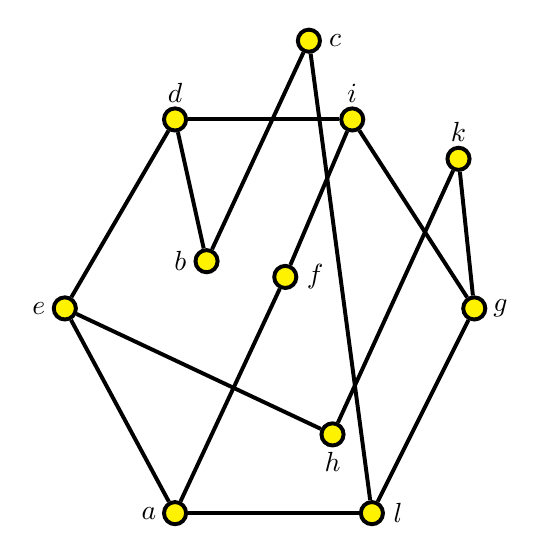
\begin{tikzpicture}
        [scale=1,every node/.style={draw,shape=circle,fill=yellow,inner sep=0,minimum size=8pt}, every path/.style={line width=0.5mm}]

        \node[label=left:{\(a\)}] (v1) at (-1.4, -3) {};
        \node[label=left:{\(b\)}] (v2) at (-1, 0.2) {};
        \node[label=right:{\(c\)}] (v3) at (0.3, 3) {};
        \node[label=90:{\(d\)}] (v4) at (-1.4, 2) {};
        \node[label=left:{\(e\)}] (v5) at (-2.8, -0.4) {};
        \node[label=right:{\(f\)}] (v6) at (0, 0) {};
        \node[label=0:{\(g\)}] (v7) at (2.4, -0.4) {};
        \node[label=270:{\(h\)}] (v8) at (0.6, -2) {};
        \node[label=90:{\(i\)}] (v9) at (0.85, 2) {};
        % \node[label=left:{\(j\)}] (v10) at (-3, 3) {};
        \node[label=90:{\(k\)}] (v11) at (2.2, 1.5) {};
        \node[label=right:{\(l\)}] (v12) at (1.1, -3) {};

        \draw (v1) -- (v5);
        \draw (v1) -- (v6);
        \draw (v1) -- (v12);
        \draw (v2) -- (v3);
        \draw (v2) -- (v4);
        % \draw (v2) -- (v6);
        % \draw (v3) -- (v10);
        \draw (v3) -- (v12);
        \draw (v4) -- (v5);
        \draw (v4) -- (v9);
        % \draw (v4) -- (v10);
        \draw (v5) -- (v8);
        % \draw (v5) -- (v10);
        \draw (v6) -- (v9);
        \draw (v7) -- (v9);
        \draw (v7) -- (v11);
        \draw (v7) -- (v12);
        \draw (v8) -- (v11);

      \end{tikzpicture}
    \end{figure}
    Certainly, this subgraph is homeomorphic to the following.
    \begin{figure}[H]
      \centering
      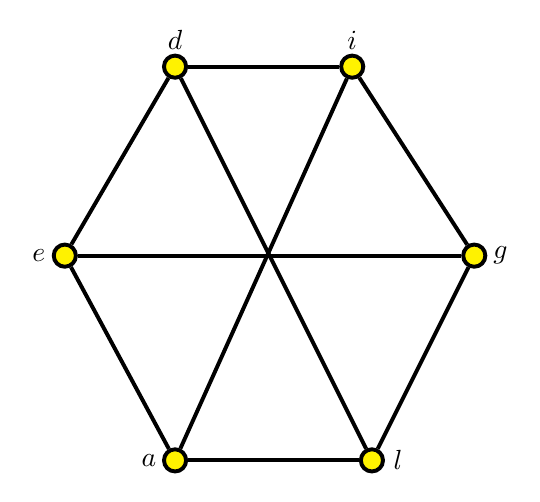
\begin{tikzpicture}
        [scale=1,every node/.style={draw,shape=circle,fill=yellow,inner sep=0,minimum size=8pt}, every path/.style={line width=0.5mm}]

        \node[label=left:{\(a\)}] (v1) at (-1.4, -3) {};
        % \node[label=left:{\(b\)}] (v2) at (-1, 0.2) {};
        % \node[label=right:{\(c\)}] (v3) at (0.3, 3) {};
        \node[label=90:{\(d\)}] (v4) at (-1.4, 2) {};
        \node[label=left:{\(e\)}] (v5) at (-2.8, -0.4) {};
        % \node[label=right:{\(f\)}] (v6) at (0, 0) {};
        \node[label=0:{\(g\)}] (v7) at (2.4, -0.4) {};
        % \node[label=270:{\(h\)}] (v8) at (0.6, -2) {};
        \node[label=90:{\(i\)}] (v9) at (0.85, 2) {};
        % \node[label=left:{\(j\)}] (v10) at (-3, 3) {};
        % \node[label=90:{\(k\)}] (v11) at (2.2, 1.5) {};
        \node[label=right:{\(l\)}] (v12) at (1.1, -3) {};

        \draw (v1) -- (v5);
        % \draw (v1) -- (v6);
        \draw (v1) -- (v12);
        \draw (v1) -- (v9);
        % \draw (v2) -- (v3);
        % \draw (v2) -- (v4);
        % \draw (v2) -- (v6);
        % \draw (v3) -- (v10);
        % \draw (v3) -- (v12);
        \draw (v4) -- (v5);
        \draw (v4) -- (v9);
        \draw (v4) -- (v12);
        % \draw (v4) -- (v10);
        % \draw (v5) -- (v8);
        % \draw (v5) -- (v10);
        \draw (v5) -- (v7);
        % \draw (v6) -- (v9);
        \draw (v7) -- (v9);
        % \draw (v7) -- (v11);
        \draw (v7) -- (v12);
        % \draw (v8) -- (v11);

      \end{tikzpicture}
    \end{figure}
    This is isomorphic to \(K_{3, 3}\) as shown below.
    \begin{figure}[H]
      \centering
      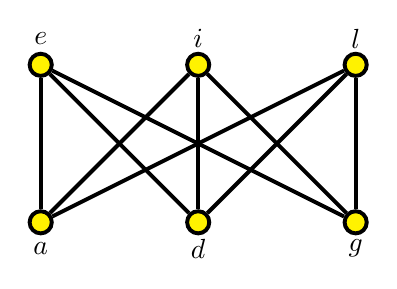
\begin{tikzpicture}
        [scale=1,every node/.style={draw,shape=circle,fill=yellow,inner sep=0,minimum size=8pt}, every path/.style={line width=0.5mm}]

        \node[label=270:{\(a\)}] (v1) at (0, 0) {};
        % \node[label=left:{\(b\)}] (v2) at (-1, 0.2) {};
        % \node[label=right:{\(c\)}] (v3) at (0.3, 3) {};
        \node[label=270:{\(d\)}] (v4) at (2, 0) {};
        \node[label=90:{\(e\)}] (v5) at (0, 2) {};
        % \node[label=right:{\(f\)}] (v6) at (0, 0) {};
        \node[label=270:{\(g\)}] (v7) at (4, 0) {};
        % \node[label=270:{\(h\)}] (v8) at (0.6, -2) {};
        \node[label=90:{\(i\)}] (v9) at (2, 2) {};
        % \node[label=left:{\(j\)}] (v10) at (-3, 3) {};
        % \node[label=90:{\(k\)}] (v11) at (2.2, 1.5) {};
        \node[label=90:{\(l\)}] (v12) at (4, 2) {};

        \draw (v1) -- (v5);
        % \draw (v1) -- (v6);
        \draw (v1) -- (v12);
        \draw (v1) -- (v9);
        % \draw (v2) -- (v3);
        % \draw (v2) -- (v4);
        % \draw (v2) -- (v6);
        % \draw (v3) -- (v10);
        % \draw (v3) -- (v12);
        \draw (v4) -- (v5);
        \draw (v4) -- (v9);
        \draw (v4) -- (v12);
        % \draw (v4) -- (v10);
        % \draw (v5) -- (v8);
        % \draw (v5) -- (v10);
        \draw (v5) -- (v7);
        % \draw (v6) -- (v9);
        \draw (v7) -- (v9);
        % \draw (v7) -- (v11);
        \draw (v7) -- (v12);
        % \draw (v8) -- (v11);

      \end{tikzpicture}
    \end{figure}
    By Kuratowski's Theorem, the graph is not planar.
  \end{solution}

  % Problem 2
  \begin{problem}
    Exhibit a planar drawing of an Eulerian planar graph with 10 vertices and 21 edges.
  \end{problem}

  \begin{solution}
        The graph shown below is planar, has the specified number of edges and vertices, and has an Eulerian circuit as follows: (1, 3, 6, 10, 9, 8, 7, 4, 8, 5, 9, 6, 5, 4, 2, 5, 3, 2, 1, 10, 7)
    \begin{figure}[ht]
      \centering
      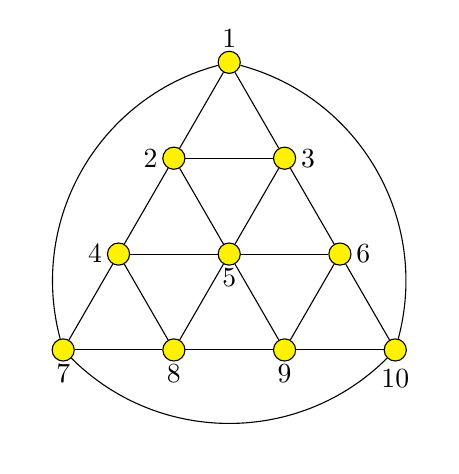
\begin{tikzpicture}
        [scale=1,every node/.style={draw,shape=circle,fill=yellow,inner sep=0,minimum size=8pt}]

        \node[label=90:{1}] (1) at (0, 0) {};
        \path (1) ++(240:40pt) node (2)[label=180:{2}] {};
        \path (1) ++(300:40pt) node (3)[label=0:{3}] {};
        \path (2) ++(240:40pt) node (4)[label=180:{4}] {};
        \path (2) ++(300:40pt) node (5)[label=270:{5}] {};
        \path (3) ++(300:40pt) node (6)[label=0:{6}] {};
        \path (4) ++(240:40pt) node (7)[label=270:{7}] {};
        \path (4) ++(300:40pt) node (8)[label=270:{8}] {};
        \path (5) ++(300:40pt) node (9)[label=270:{9}] {};
        \path (6) ++(300:40pt) node (10)[label=270:{10}] {};

        \draw (1) -- (2);
        \draw (1) -- (3);
        \draw (2) -- (3);
        \draw (2) -- (4);
        \draw (2) -- (5);
        \draw (3) -- (5);
        \draw (3) -- (6);
        \draw (4) -- (5);
        \draw (4) -- (7);
        \draw (4) -- (8);
        \draw (5) -- (6);
        \draw (5) -- (8);
        \draw (5) -- (9);
        \draw (6) -- (9);
        \draw (6) -- (10);
        \draw (7) -- (8);
        \draw (8) -- (9);
        \draw (9) -- (10);
        \draw [bend right=45] (1) to (7);
        \draw [bend right=45] (7) to (10);
        \draw [bend right=45] (10) to (1);

      \end{tikzpicture}
    \end{figure}
  \end{solution}

  % Problem 3
  \begin{problem}
    We say that a relation \(R\) on a set \(X\) is symmetric if \(\left( x, y\right) \in R\) implies \(\left(y, x\right) \in R\) for all \(x, y \in X\). If \(X = \{ a, b, c, d, e, f \}\), how many symmetric relations are there on \(X\)? How many of these are reflexive?
  \end{problem}

  \begin{solution}
    A relation \(R\) is merely a subset of \(X \times X\). If \(|X| = n\), \(R\) is a subset of a set with \(n^{2}\) elements. If \(R\) is symmetric, then the elements of \(R\) can be treated as sets of size 2 since the order does not matter. These sets can be formed by choosing 2 elements out of \(n\). That is, elements of \(R\) can be selected from a set of size \({n \choose 2}\). However, this excludes elements of the form \(\left(a, a\right)\). To account for these, we add \(n\) more ordered pairs to our set of size \({n \choose 2}\). Thus, \(R\) is a subset of a set of size \({n \choose 2} + n = \frac{n(n+1)}{2}\). Therefore, there are \(2^{\frac{n(n+1)}{2}}\) symmetric relations on \(X\).


    A relation \(R\) is reflexive if for every \(a \in X\), \(\left(a, a\right) \in R\). Thus, \(R\) must contain the \(n\) ordered pairs of that form. Then \(R\) is a subset of a set containing the remaining \(n^{2} - n = n \left(n - 1\right)\) relations. Thus, there are \(2^{n \left(n - 1\right)}\) reflexive relations on \(X\).
  \end{solution}
\end{document}
